%\textcolor{blue}{My\_First\_FFT\_code.m}
%\chapter{Version 3.0: some big changes}


\chapter{The big changes}

For this new version of OSCAR the code has been totally rewritten using the Oriented Object capability of Matlab. The code is now more user friendly and less prone to errors. Moreover some new functions has been added and the higher order optical modes are supported from the start.

The principle of the FFT code and the method to derive results are still unchanged, so for people not familiar with FFT code, it is strongly recommended to read the first part of this manual.

\paragraph{Requirements} The new OSCAR works with Matlab version superior to 2009a and the \textsl{Optimization Toolbox} is necessary if beam fitting functions are used.

\section{Motivation and goals}

 First, the curious reader may wonder why there is no version 2.0 of OSCAR. Such a version exists, it is OSCAR classic with the implementation of a power recycled Michelson with Fabry Perot arm cavities. This version was developed to simulated LIGO-Virgo type of interferometers but was never officially distributed.

 The code of version 2.0 was becoming messy since OSCAR was not intended to be so advanced (remember, it was only supposed to simulate the test cavity at Gingin in Australia). To include all the code developed for the version 2.0, it was decided to write a full new version of OSCAR taking also into account all what I learned as a OSCAR user.

 Doing a new version allowed some radical changes: no more global variables, add change of refractive index, sidebands field managed automatically at the same time as the carrier, manage higher order modes and much more\dots In the long term OSCAR should be able to simulate Advanced gravitational wave detectors with realistic optics and that in a very simple script.

 The new code should also take into account the computing progress made in recent years. For example, the version 3.0 has been written with parallel processing in mind, for example the North and West arms could be computed in parallel on different cores of the CPU (the Parallel Processing Toolbox is then required) or a cavity scan can use up to 8 cores. Calculations on the GPU will also be integrated (when I get suitable computer).

 The new code can also use separate grid size in the same simulation. That could be used to simulate non degenerated recycling cavities, where the laser beam has to be strongly focused and could change size by a factor 10.

\section{The new objects and how to use them}

The main change of this version for the user is the use of Oriented Object programming for OSCAR. A laser field or a mirror are no longer complex 2D matrices but are objects with different attributes. Each object is part of a class, for example the laser beam is an instance of the class \textsl{E\_field}, a mirror surface is an object from the class \textsl{Interface}. Functions are defined to work on specific class and not on any random 2D data.

The definition of the classes and their associated functions are presented in the following subsections. In the description of the function call, argument and output variables in \textbf{bold} are mandatory. For more detailed descriptions of the functions and the associated syntax, the help of Matlab can be used (help followed by the name of the function).

\subsection{The class Grid}
\textbf{G1} = \textcolor{blue}{Grid}(Nb\_points\_grid,Size\_grid)
by default: Nb\_points\_grid~=~256 and Size\_grid~=~1 \\

The class \textsl{Grid} is used to represent the discretisation of the space and all the associated variables (see \ref{App3:grid} for the details). It was formerly known as the global variable \textsl{Grid} in OSCAR classic. One \textsl{Grid} object is the first object to be defined in a OSCAR script. To define an instance of the class \textsl{Grid}, 2 parameters are necessary: the number of pixels used (typically 128 or 256) and the size of the grid in meter. For example:

\begin{verbatim}
G1 = Grid(128,0.40);
\end{verbatim}

Define the object \textsl{G1} of the class \textsl{Grid}, then later all the objects for the simulations will be defined on a grid of $128 \times 128$ with a side length of 40~cm.

Only one function is associated with the class \textsl{Grid}, it is \textcolor{blue}{What\_is\_possible}. \textcolor{blue}{What\_is\_possible}(\textbf{G1}) returns for the grid \textsl{G1} what is the maximum curvature or tilt for a mirror of diameter \textsl{diam}. By default the mirror diameter is 80\% of the size of the grid and the wavelength is set to 1064~nm.

It is is possible to change manually the diameter of the mirror and the wavelength of the laser by using the optional arguments \emph{'diam'} and \emph{'wavelength'}: \verb? What_is_possible(G1,'diam',0.2,'wavelength',633E-9) ?

\noindent \textbf{map2D} = \textcolor{blue}{Do\_Virtual\_map}(\textbf{G}, \textbf{Power\_law})
\vspace*{-0.2cm}
\begin{quote}
Function to create a synthetic map from a given PSD. The PSD is parameterized as a (or several) power law. The function return a 2D height map of the surface which can then after be applied to a Interface object. See the example \textcolor{blue}{Example\_Display\_Create\_maps.m} for a practical implementation.
\end{quote}


\subsection{The class E\_field}
\textbf{E1} = \textcolor{blue}{E\_field}( \textbf{Grid\_name} , \emph{options}) by default the laser beam is in the fundamental mode

Instances of the class \textsl{E\_field} are laser beams, represented as electric field in a complex 2D matrix. The objects \textsl{E\_field} contain a wavelength (1064 nm by default) and also the refractive index of the medium where the laser beam is. If sidebands are present, they are also implemented in the object at the same time as the carrier. All the variables and parameters of objects \textsl{E\_field} are detailed in \ref{App3:E_field}.

Since OSCAR version 3.05, there is now different ways to define a laser beam:
\begin{itemize}
  \item with the waist: \\
        \verb? E_input = E_Field(G1,'w0',0.02) ?
  \item with the waist and a distance: \\
        \verb? E_input = E_Field(G1,'w0',0.02,'z',-10) ?
  \item with a beam radius and a wavefront curvature: \\
        \verb? E_input = E_Field(G1,'w',0.018,'R',-1420) ?
  \item with the complex q parameter: \\
        \verb? E_input = E_Field(G1,'q',12 + 1200*1i) ?
  \item the optical mode can also be specified, for example for a helicoidal mode LG 3 3:
        \verb? E_input = E_Field(G1,'w0',0.02,'mode','LG_HELI 3 3') ?
        To define the mode basis, 3 options are possible: 'HG n m', 'LG\_HELI n m' or 'LG\_SIN n m'
\end{itemize}
A non distributed function exist also to create astigmatic beam. Most of OSCAR's functions are applied to objects of this class. The essential functions are described below:\\

\noindent \textbf{E2} = \textcolor{blue}{Add\_HOM}(\textbf{E1}, \textbf{max\_mode\_order})
\vspace*{-0.2cm}
\begin{quote}
Add some higher order optical modes to a fundamental mode. It is possible to choose the power distribution of the higher order modes.
\end{quote}

\noindent \textbf{E2} = \textcolor{blue}{Add\_sidebands}(\textbf{E1}, \textbf{mod freq}, \textbf{mod index})
\vspace*{-0.2cm}
\begin{quote}
Create two frequency shifted sidebands fields from a carrier E\_Field \textsl{E1} as the phase modulator would do in the optic lab. The separation frequency between the carrier and the sideband is given by \textsl{mod freq}, and the modulation index by \textsl{mod index}. At present in OSCAR, no sidebands of sidebands is allowed.
\end{quote}

\noindent overlap = \textcolor{blue}{Calculate\_Overlap}(\textbf{E1,E2})
\vspace*{-0.2cm}
\begin{quote}
Calculate the overlap integral between 2 E\_field. The function returns the complex normalised overlap between the 2 fields. Without any output argument, the function returns in the command window the power coupling (i.e. square of the absolute value of the overlap integral) between the field E1 and E2.
\end{quote}

\noindent overlap = \textcolor{blue}{Calculate\_Overlap\_SB\_Car}(\textbf{E1})
\vspace*{-0.2cm}
\begin{quote}
Calculate the overlap integral between the carrier and the lower and upper sidebands for one E\_field. The function returns two complex normalised numbers which are the overlap between the carrier and the two sidebands. Without any output argument, the function returns in the command window the power coupling (i.e. square of the absolute value of the overlap integral).
\end{quote}

\noindent power = \textcolor{blue}{Calculate\_power}(\textbf{E1},'include','carrier'|'all'|'SB')
\vspace*{-0.2cm}
\begin{quote}
Calculate the total power of the E\_Field \textsl{E1}. The function can either return a number or display the value in the Matlab command line if no output variable is used. A similar function \textcolor{blue}{Calculate\_power\_SB} exists to calculate the power of the sidebands fields.
To simulate a DC photodiode, which will sum all the field frequencies, one can use  \textcolor{blue}{Calculate\_power}(E1,'include','all').
\end{quote}

\noindent \textbf{E2} = \textcolor{blue}{Change\_E\_n}(\textbf{E1},\textbf{n})
\vspace*{-0.2cm}
\begin{quote}
Change the refractive index where the laser beam is. Could be use to pass through a flat interface from a vacuum to a mirror substrate for example.
\end{quote}

\noindent return\_param = \textcolor{blue}{Check\_pos\_tilt}(\textbf{E1})
\vspace*{-0.2cm}
\begin{quote}
Use as a diagnostic tool to check the centroid position of the beam on the grid as well as its tilt, function in both directions at the same time.
\end{quote}

\noindent [\textbf{sig\_p sig\_q}] = \textcolor{blue}{Demodulate\_SB}(\textbf{E1})
\vspace*{-0.2cm}
\begin{quote}
Demodulate the field \textsl{E1} with the present pair of sidebands. As the result, the in phase \textsl{sig\_p} and in quadrature \textsl{sig\_q} signals are given. This function could be used to derive a Pound Drever Hall error signal as shown in \ref{ch4:ex_PDH}.
\end{quote}

\noindent Mat\_scattered = \textcolor{blue}{Expand\_HOM}(\textbf{E1},\textbf{max\_mode\_order})
\vspace*{-0.2cm}
\begin{quote}
Expand the beam \textsl{E1} into the Hermitte Gauss basis defined by \textsl{E1} (\textsl{E1} must be close to a fundamental mode). The result is given as the normalised power content in the different optical modes. If not output is given a plot is made. Several options are possible:
\end{quote}
\begin{itemize}
  \item to output all the power content into the different higher order modes up to the order 10 \\
        \verb? Expand_HOM(E1,10,'display','pyramid') ?
  \item to define a different basis for the calculation given as beam radius and complex wavefront curvature in meter\\
        \verb? Expand_HOM(E1,10,'basis',[0.05 -1400]) ?
\end{itemize}


\noindent \textcolor{blue}{E\_plot}(\textbf{E1})
\vspace*{-0.2cm}
\begin{quote}
Display a 2D plot of the field amplitude in a new Matlab figure window. Function can also be used as \textsl{E1}.E\_plot(). We can also display the amplitude in log scale \verb?E_plot(E1,'space','log')? or the propagating angle of the beam \verb?E_plot(E1,'angle')?. To create illustrative picture of the beam without all the axis, one can use the option \verb?'no_axis',true?.

A similar function exist also for the sidebands (but with less options): \noindent \textcolor{blue}{E\_plot\_SB}
\end{quote}


\noindent [beam\_radius wavefront\_RofC] = \textcolor{blue}{Fit\_E\_Field}(\textbf{E1})
\vspace*{-0.2cm}
\begin{quote}
This function is used to find the beam parameter of the field \textsl{E1}, it can also be used for higher order modes. If no output are given the result is written in the Matlab command window. To fit only the fundamental mode, it is faster to use the function \textcolor{blue}{Fit\_TEM00}.

For the fit of an astigmatic fundamental mode, it is recommended to use the function \textcolor{blue}{Fit\_TEM00\_xy}.
\end{quote}


\noindent [\textbf{Eout},\textbf{Gout}] = \textcolor{blue}{Focus\_beam\_with\_telescope}(\textbf{Ein},\textbf{array\_L\_D})
\vspace*{-0.2cm}
\begin{quote}
With this function, one can now simulate mirrors with small radius of curvature to simulate strongly focused beam. The method has been inspired by the work done J.Y. Vinet \cite{Virgo_PB} and H. Yamamoto \cite{Hiro1}.
The new function can dynamically adapt the size of the grid and as such the focused beam is defined on a new grid. This function is used to simulate the focusing mode matching telescope at the input or output of the interferometer.
The input argument is the input field and a vector with the focal length of the equivalent mirror/lens and the separation between the optical elements in meters. A telescope with several lenses can be simulated with only one call of the function.
See the provided example for more details.
It has also the possibility to add maps and finite size optics to the telescope.
\end{quote}

\noindent \textbf{E2} = \textcolor{blue}{Normalise\_E}(\textbf{E1},power)
\vspace*{-0.2cm}
\begin{quote}
Normalise the E\_field \textsl{E1} to 1~W if no \textsl{power} argument is specified. Only the carrier is affected by this function and not the sidebands.
\end{quote}

\noindent \textbf{E2} = \textcolor{blue}{Propagate\_E}(\textbf{E1},\textbf{dist})
\vspace*{-0.2cm}
\begin{quote}
Propagate the field \textsl{E1} over a distance \textsl{dist} in meter. If sidebands are present, the sidebands are automatically propagated at the same time, with of course the adequate phase shift.
\end{quote}

\noindent \textbf{E2} = \textcolor{blue}{Reflect\_mirror}(\textbf{E1},\textbf{I1})
\vspace*{-0.2cm}
\begin{quote}
Returns the field after reflection on a mirror. \textsl{I1} is an Interface object which must have been previously defined. An alternative syntax could be \textcolor{blue}{Reflect\_mirror}(\textbf{E1},\textbf{R1}), with \textsl{R1} the radius of curvature of the mirror to be reflected on. A concave mirror is represented by a positive \textbf{R1}.

Reflections inside the substrates are allowed since the index of refraction is taken into account for the reflection.
\end{quote}


\noindent E3 = \textcolor{blue}{ Remove\_00\_part}(\textbf{E1},E2)
\vspace*{-0.2cm}
\begin{quote}
Remove the fundamental Gaussian part from a field \textbf{E1}. That is useful to see which higher order modes are superposed with the fundamental mode following some cavities simulations. Can also be used to subtract 2 fields E1 and E2 as in the case of destructive interferences.
\end{quote}


\noindent \textbf{E2} = \textcolor{blue}{Transmit\_Aperture}(\textbf{E1},\textbf{size}, 'circle' $\mid$ 'square')
\vspace*{-0.2cm}
\begin{quote}
Transmit the field \textsl{E1} through an aperture of diameter \textsl{size}. The aperture could be round or square, if not specified it is round. Custom aperture can also be defined see the function help for example.
\end{quote}

\noindent \textbf{E2} = \textcolor{blue}{Transmit\_lens}(\textbf{E1},\textbf{focal length})
\vspace*{-0.2cm}
\begin{quote}
Transmit the field \textsl{E1} through a lens of a given focal length.
\end{quote}

\noindent [\textbf{E\_trans} E\_ref]= \textcolor{blue}{Transmit\_Reflect\_Interface}(\textbf{E1},\textbf{I1})
\vspace*{-0.2cm}
\begin{quote}
Transmit and reflect the field \textsl{E1} through an interface \textsl{I1}. The orientation of the interface is given by the refractive index of the incoming field \textsl{E1}.
\end{quote}

For convenience, the operators +,- and * have also been overloaded to work with any object \textsl{E\_field}.

\subsection{The class Prop\_operator}
\label{Sec:DI}
This is an internal class which must be almost invisible for the user. The objects of this class allows to speed up the propagation of electrical field \textsl{E\_Field} thanks to the pre-calculation of the propagation matrix. A \textsl{Prop\_operator} is automatically created when a cavity is created. It represents the propagation operator over one cavity length.

Since OSCAR 3.10, a new method of propagation has been implemented based on the method of digital integration \cite{DI_paper}. This method is slower, however it eliminates the light leaking out from the simulation grid. With the direct implementation, a minimal distance of propagation is essential for the validity of this technique. The distance depends on the size of the grid and can be checked with the function \textcolor{blue}{What\_is\_possible}.

To enable the digital integration, one has to set the logical variable \textsl{Prop\_operator.Use\_DI} to true. For example, to use the digital integration for the simulation of the cavity \textsl{C1}, we will write:

\verb? C1.Propagation_mat.Use_DI = true; ?

The parameters included in the class \textsl{Prop\_operator} are described in \ref{App3:Prop_OP}\\


The creator for this class is:

\noindent \textbf{Prop} = \textcolor{blue}{Prop\_operator}(\textbf{Grid\_name},\textbf{Length}, n)

\vspace*{-0.2cm}
\begin{quote}
The variable \textsl{Length} represents the propagation length in meter. One can also specify an optional parameter \textsl{n}, the refractive index of the media, that way, thick substrate can also be implemented.
\end{quote}
To propagate a laser beam (and its sidebands) one can simply use:

\verb?  E2 = Propagate_E(E1, Prop) ?

\subsection{The class Interface}
\textbf{I1} = \textcolor{blue}{Interface}(\textbf{Grid\_name},options)

The class \textsl{Interface} is used to represent a surface which separates two media of refractive index. Objects of this class are used to represent mirrors, lenses or curved interfaces between air and glass. The structure of the class \textsl{Interface} is described in \ref{App3:Inter}.

To define a concave mirror for a laser beam, the radius of curvature must be positive. Internally in OSCAR, the sagitta of the surface view from the medium n1 toward n2 will be negative by convention. The surface is stored in the variable \textsl{I1.surface}.

Below are some ways to define an interface:
\begin{itemize}
  \item Interface to define a curved surface of radius 1000~m between the refractive 1 and 1.45 \\
        \verb?  Interface(Grid,'RoC',1E3,'n1',1,'n2',1.45) ?
  \item a mirror with an aperture of 20~cm of diameter \\
      \verb?  Interface(Grid,'RoC',1E3,'CA',0.2) ?
   \item a mirror with an aperture of 20~cm of diameter and angle of incidence of 3 degrees \\
      \verb?  Interface(Grid,'RoC',1E3,'CA',0.2,'AoI',3) ?
  \item add the transmission of 1\% and loss of 50 ppm\\
        \verb?  Interface(Grid,'RoC',1E3,'CA',0.2.'T',0.01,'L',50E-6) ?
\end{itemize}
The options can be defined in any order. To define flat mirrors, a \verb?'RoC'? of \verb?0 or Inf? can be used. Check the file \verb?@Interface/Interface.m? to see the default parameters.

The list of methods associated with the objects of the class \textsl{Interface} is given below:

\noindent \textbf{I2} = \textcolor{blue}{Add\_astigmatism}(\textbf{I1}, \textbf{Zernike amplitude}, \textbf{Diameter})
\vspace*{-0.2cm}
\begin{quote}
Add to the surface of the interface \textsl{I1} the Zernike polynomial 2,2 (which represents the astigmatism) with an amplitude of \textsl{Zernike amplitude} and over a diameter \textsl{Diameter}.
\end{quote}


\noindent \textbf{I2} = \textcolor{blue}{Add\_map}(\textbf{I1}, \textbf{filename}, options)
\vspace*{-0.2cm}
\begin{quote}
Add to the surface of the interface \textsl{I1} a square map loaded from the file \textsl{filename}. For square maps, the resolution of one pixel must be given by the parameters \verb?'reso'?. The map can also be normalised to a certain RMS using the option \verb?'RMS'? or the height can be scaled by scalar with the option \verb?'scale'?. One can also rotate the map by a number of time 90 degrees with the option \verb?'rotate'?. The option \verb?'remove the tilt and focus'? can remove the tilt focus from the added map. The tilt/focus is removed over all the surface but with the optimal calculated only over a diameter.

Here some examples:
\begin{itemize}
  \item load the file map1.dat \\
        \verb? I1 = Add_map(I1,'map1.dat','reso',3.5E-4) ?
  \item load the map and scale it to 1 nm RMS \\
        \verb? I1 = Add_map(I1,'map1.dat','reso',3.5E-4,'RMS',1E-9) ?
  \item rotate the map by 90 degree \\
        \verb? I1 = Add_map(I1,'map1.dat','reso',3.5E-4,'rotate',1) ?
  \item remove the tilt and focus \\
         \verb? I1 = Add_map(I1,'map1.dat','reso',3.5E-4,'remove_tilt_focus',0.150) ?
\end{itemize}

Maps with cylindrical symmetry can be loaded as a 2 columns text file. First column is the radius and the second is the height in meter. In that case the resolution does not have to be specified. To supress the output, the option \verb?'verbose',false? can be used. A new experimental argument is \verb?'centering'? to offset the map if this region of interest is not at the center.
\end{quote}


\noindent \textbf{I2} = \textcolor{blue}{Add\_tilt}(\textbf{I1}, \textbf{tilt\_angle}, 'x')
\vspace*{-0.2cm}
\begin{quote}
Tilt the whole surface of the interface \textsl{I1} by the amount \textsl{tilt\_angle} in radian. It is possible to specify the direction of the tilt by setting the third argument \textsl{'x'} or \textsl{'y'}. By default the tilt is in the vertical direction (recommended solution).
\end{quote}


\noindent \textbf{I2} = \textcolor{blue}{Cut\_frequency\_Interface}(\textbf{I1},\textbf{Option},\textbf{f\_cut})
\vspace*{-0.2cm}
\begin{quote}
Remove given spatial frequency within a given interface object. The argument \textsl{Option} is a string \verb?'LP'?, \verb?'HP'? or \verb?'BP'? for respectively low pass, high pass or band pass filter. \textsl{f\_cut} is the cutting spatial frequency in m$^{-1}$, for band pass filtering \textsl{f\_cut} is vector of two frequencies.\\
The implementation for the filtering is done in a straight forward manner (see the simple code), so as a result artefact may appear in the resulting object \textsl{I2}.
\end{quote}


\noindent I2 = \textcolor{blue}{Expand\_Zernike}(\textbf{I1},options)
\vspace*{-0.2cm}
\begin{quote}
Expand in Zernike polynomials the interface \textsl{I1}. Two options are available: 'Z\_order', an integer which represents the maximum order of the Zernike polynomials to take in to account in the calculations and 'diam', the diameter where the Zernike polynomials are defined. This function returns the interface \textsl{I2}, which is the interface reconstructed by the Zernike polynomials. Example:
\verb? I2 = Expand_Zernike(I1,'Z_order',10,'diam',0.2) ?
\end{quote}


\noindent \textcolor{blue}{I\_plot}(\textbf{I1})
\vspace*{-0.2cm}
\begin{quote}
Plot the surface of the interface \textsl{I1}. The color scale is in meter. \verb? I_plot(I1,'diam',0.160)? will only plot the surface over a diameter of 160mm.
\end{quote}


\noindent \noindent [\textbf{PSD\_1D} \textbf{freq}] = \textcolor{blue}{Plot\_PSD}(\textbf{I1}, options)
\vspace*{-0.2cm}
\begin{quote}
Function used to calculate the one dimension Power Spectral Density (PSD) of a surface. The two output arguments are the vector of the PSD and the vector of the frequency. By default before calculating the PSD 2D, a Hanning window is applied to the data and the PSD is calculated summing all the frequencies over one direction to pass from 2D to 1D. A detailed explanation of the different ways to calculate the PSD can be found in a Hiro LIGO note \cite{Hiro_PSD}.

An example for the possible options can be found below, combination of the different options is allowed:
\begin{itemize}
  \item Calculate the PSD over a given diameter, given in meter \\
        \verb? [PSD_1 freq] = Plot_PSD(I1,'diam',0.150) ?
  \item Calculate the PSD by summing radial frequencies \\
        \verb? [PSD_1 freq] = Plot_PSD(I1,'rect_1D',false) ?
  \item Use a Gaussian weighting to calculate the PSD, must input the Gaussian beam radius (in meter) \\
        \verb? [PSD_1 freq] = Plot_PSD(I1,'window_Gaussian',0.05) ?
  \item Plot directly the PSD in the current window \\
        \verb? [PSD_1 freq] = Plot_PSD(I1,'display',true) ?
\end{itemize}
\end{quote}


\noindent RMS = \textcolor{blue}{Weighted\_RMS}(\textbf{I1,Ein})
\vspace*{-0.2cm}
\begin{quote}
Calculate the RMS of the surface \textsl{I1} weighted by the intensity of the field \textsl{Ein}. A diameter can also be given as the second argument. Beware the curvature is not subtracted before the calculation, so a perfectly curved spherical mirror will have a non zero RMS.
\begin{itemize}
  \item Calculate the weighted RoC \\
        \verb? RMS = Weighted_RMS(I1,E_Field(G1,'w',0.05)) ?
  \item Display directly the calculated RMS \\
        \verb? Weighted_RMS(I1,0.2) ?
\end{itemize}
\end{quote}


\noindent RoC\_fitted = \textcolor{blue}{Weighted\_RoC}(\textbf{I1,Ein})
\vspace*{-0.2cm}
\begin{quote}
Calculate the radius of curvature of the surface \textsl{I1} weighted by the intensity of the field \textsl{Ein}. This calculation is useful to fit non perfectly spherical surface. A diameter can also be given as the second argument.
\begin{itemize}
  \item Calculate the weighted RoC \\
        \verb? RoC = Weighted_RoC(I1,E_Field(G1,'w',0.05)) ?
  \item Display directly the radius of curvature \\
        \verb? Weighted_RoC(I1,0.2) ?
\end{itemize}
\end{quote}

The operators \verb?+?,\verb?-? have also been overloaded to be used with object of the class \textit{Interface}.

\subsection{The class Mirror}
\textbf{M} = \textcolor{blue}{Mirror}( \textbf{I\_HR}, \textbf{I\_AR}, \textbf{Substrate\_length})

This class can simulate thick substrates. The substrate can be part of a cavity as an input mirror for example. If the substrate is part of the cavity, the surface \textsl{I\_HR} is supposed to be the HR coating (and hence inside the cavity).

\textsl{I\_HR} and \textsl{I\_AR} are 2 objects of the class \textsl{Interface}. The 2 interfaces must share the same refractive index superior to 1. \textsl{Substrate\_length} is a scalar used to represent the thickness of the substrate in meter.

The mirror object can also be used to simulate the etalon effect. Indeed if the AR surface is imperfect (R\_AR $>$ 0), light can be bounced several times within the substrate before exiting. The number of round trip is hard-coded but can be changed using the line (by default it is 1):

 \verb? M.RT_inside=3 ?

Two similar procedures can be used with the class \textsl{Mirror}. The procedures simulate the transmission and reflection of an E\_field by an instance of the class \textsl{Mirror}:

\noindent [\textbf{E\_trans} E\_ref]= \textcolor{blue}{Transmit\_Reflect\_Mirror}(\textbf{E1},\textbf{M1},'AR')
\vspace*{-0.2cm}
\begin{quote}
Calculate the transmitted and reflected fields (\textsl{E\_trans} and \textsl{E\_ref} respectively) by an object \textsl{M1} of the class Mirror. The input beam is \textsl{E1}. The first interface to consider, indicating the direction of the incoming beam can be either the HR or AR surfaces according to the last argument 'HR' or 'AR' .
\end{quote}

A new function \textcolor{blue}{Transmit\_Reflect\_Optic} has also been created which can be used by either Interface object or Mirror object. Internally, this function calls the function \textcolor{blue}{Transmit\_Reflect\_Interface} or \textcolor{blue}{Transmit\_Reflect\_Mirror} depending on the input parameters.

\subsection{The class Cavity1}
\textbf{C1} = \textcolor{blue}{Cavity1}( \textbf{I1}, \textbf{I2}, \textbf{Cavity\_length}, \textbf{E1})

This class is used to simulate Fabry Perot cavities. Objects of the class \textsl{Cavity1} are cavities constituted by two Interface objects \textsl{I1, I2} separated by a distance \textsl{Cavity\_length}. An input field \textsl{E1} must also be given. \textsl{I1} is considered as the input surface where the input beam is defined, whereas \textsl{I2} is the end mirror.

The input field can be defined either inside the cavity on the surface \textsl{I1} or outside the cavity. In the later case, the input beam will first be transmitted through \textsl{I1} which can act as a lens. By default the input beam is defined inside the cavity, if it is not the case the user can add in his script:
\begin{verbatim}
C1.Laser_start_on_input = false ;
\end{verbatim}

Variables of instances of the class \textsl{Cavity1} are listed in {App3:Cavity}.

\noindent Several functions are associated with the class \textsl{Cavity1}:

\noindent \textbf{Cout} = \textcolor{blue}{Calculate\_fields}(\textbf{Cin})
\vspace*{-0.2cm}
\begin{quote}
\textcolor{blue}{Calculate\_fields} calculates the fields on resonance inside the cavity and stored them for future use. Compared to \textcolor{blue}{Get\_info} this function also calculates the reflected field, so the input laser beam has can not be defined inside the cavity. The results can be displayed using \textcolor{blue}{Display\_results}(Cout).
Before the finding the steady state fields inside the cavity, the cavity working point (i.e the resonance condition) has to be set, for example using the function \textcolor{blue}{Cavity\_resonance\_phase}.
With the option argument \verb?'iter'? or \verb?'accuracy'?, one can set the level of accuracy (and hence the computational time) for the simulation.
\end{quote}

\noindent \textbf{Cout} = \textcolor{blue}{Calculate\_fields\_AC}(\textbf{Cin})
\vspace*{-0.2cm}
\begin{quote}
\textcolor{blue}{Calculate\_fields\_AC} is similar to the function \textcolor{blue}{Calculate\_fields} except it used the accelerated convergence scheme \cite{Saha:97,DAY_AC} to find the steady state fields inside the cavity. The gain in speed could be important if the cavity is close to a perfect cavity, so the steady field is near a perfect fundamental mode.
This function works for the carrier and for the sideband fields, if present. Also for a better convergence it is recommended to use the digital integration method for the propagation of the field (see \ref{Sec:DI}).
A second function \textcolor{blue}{Calculate\_fields\_AC2} using another more advanced convergence scheme which can give more accurate results.
\end{quote}

\noindent \textbf{Cout} = \textcolor{blue}{Calculate\_RT\_mat}(\textbf{Cin})
\vspace*{-0.2cm}
\begin{quote}
Calculate the round trip kernel of the cavity for the electrical field. This is later use to calculate the cavity eigenmodes and eigen values. The kernel itself is a 2D complex matrix of size \textsl{Nb\_points}$^2$ $\times$ \textsl{Nb\_points}$^2$, so the kernel can real take out a lot of memory. On a desktop, one might want to limit textsl{Nb\_points} to 64, while on a powerful desktop one can go up to 128.

To calculate the kernel, the digital integration technique has to be used for the beam propagation. This technique to be valid required a minimum propagation distance which depends on the size of the grid. If this is a problem, the kernel can be calculated on a different grid (contact the author for more details on this topic).
\end{quote}

\noindent \textbf{Cout} = \textcolor{blue}{Cavity\_lock\_PDH}(\textbf{Cin})
\vspace*{-0.2cm}
\begin{quote}
Adjust the resonance condition to minimise the error signal derived from a Pound Drever Hall locking scheme \cite{black:79}. To calculate the error signal a pair of sidebands must be present and the function \textcolor{blue}{Cavity\_resonance\_phase} must first be run.
\end{quote}

\noindent \textcolor{blue}{Check\_stability}(\textbf{Cin})
\vspace*{-0.2cm}
\begin{quote}
Calculate the radius of curvature of the input and end mirrors and then check the stability and gain of the cavity. Function useful when mirror maps with curvature are used. An optional second argument could be given to specify the diameter on which the mirror radius of curvature is calculated. For example to calculate the stability of the cavity only taking into account the central 6 cm diameter of the mirror, one can use:
\verb? Check_stability(C1,'diam',0.06) ?
The function also return the input beam parameters of the fundamental mode for a perfect mode matching.

\end{quote}

\noindent \textcolor{blue}{Check\_matching}(\textbf{Cin},nb\_RT)
\vspace*{-0.2cm}
\begin{quote}
Propagate the input beam back and forth between the cavity input and end mirrors and check the beam size before each reflection. The mode matching is good if during multiple round trips the beam size on the mirror does not fluctuate (but could be different of course on the input and end mirror). The optional argument \textsl{nb\_RT} can set the number of round trip to be done.
\end{quote}

\noindent \textbf{Cout} = \textcolor{blue}{Cavity\_resonance\_phase}(\textbf{Cin})
\vspace*{-0.2cm}
\begin{quote}
Calculate the macroscopic length tuning to bring the cavity on resonance for the input field. The cavity resonance has to be found before any calculations on the cavity (circulating fields, loss calculations,\dots) are launched. The input and output arguments are usually the same.
A second function \textcolor{blue}{Cavity\_resonance\_phase2} is also present, this function gives more accurate results when the cavity is degenerated.
\end{quote}

\noindent \textbf{Cout} = \textcolor{blue}{Cavity\_scan}(\textbf{Cin})
\vspace*{-0.2cm}
\begin{quote}
Scan the cavity over one free spectral range and then set the cavity resonance to maximise the circulating power. This procedure is much slower than \textcolor{blue}{Cavity\_resonance\_phase} but can still be useful to check if some higher order modes are excited since after the FSR scan can be displayed.
The presence of sidebands in the input beam of the cavity can also be implemented. First the sidebands have to be defined and then the option \verb? 'With_SB',true? must be added in the command.
\end{quote}

\noindent \textcolor{blue}{Display\_cavity\_modes}(\textbf{Cin},'N',10,'Airy',1)
\vspace*{-0.2cm}
\begin{quote}
Display the cavity eigen modes. The function \textcolor{blue}{Calculate\_RT\_mat} must first has been run, so the cavity kernel has been calculated. With this function one can display an arbitrary number of modes (by default the first 20) and also draw the Airy peak of the cavity with the command:

  \verb? Display\_cavity\_modes(C1,'N',30,'Airy',1) ?

An example of how to use the function \textcolor{blue}{Display\_cavity\_modes} is shown in the script \textcolor{blue}{Example\_cavity\_eigenmodes.m}
\end{quote}

\noindent \textcolor{blue}{Display\_scan}(\textbf{Cin})
\vspace*{-0.2cm}
\begin{quote}
Display the scan from a cavity after the procedure \textcolor{blue}{Cavity\_scan} was run. By moving the cursor on the upper plot (circulating power vs tuning), the profile of the optical modes can be checked in the lower right plot.
\end{quote}

\noindent \textcolor{blue}{Get\_info}(\textbf{Cin})
\vspace*{-0.2cm}
\begin{quote}
\textcolor{blue}{Get\_info} calculates the fields on resonance inside the cavity. The function is also use to calculate the diffraction loss due to the mirror finite size.
\end{quote}



\subsection{The class CavityN}

\textbf{CN} = \textcolor{blue}{CavityN}( \textbf{I}, \textbf{D}, \textbf{E1})

This class introduces linear cavity with arbitrary number of mirrors. \textsl{I} represents a vector of object Interfaces, \textsl{D} is a vector of distances and finally \textsl{E1} is the input laser field.

Two kinds of cavity could be defined:
\begin{itemize}
  \item A ring cavity where the laser beam is reflected on each mirror only once during one round trip (3 or 4 mirrors mode cleaner cavity falls in this category). In that case, the length of the vector \textsl{I} is the same as the one of \textsl{D}.
  \item A folded cavity, where during one round trip the laser beam is reflected twice by the intermediate mirrors (think recycling folded cavity of LIGO). In that case, it has one more interface \textsl{I} than length \textsl{D}.
\end{itemize}


The distance  \verb|D(n)| is defined as the distance between the interfaces  \verb|I(n)| and  \verb|I(n+1)|. The functions suitable for the class \textsl{CavityN} are the same as for the class \textsl{Cavity1} without exception.

An example of how to use the class \textsl{CavityN} is shown in the script \textcolor{blue}{Example\_4mirrors.m}

\subsection{The class Mirror}

This class is used to simulate optics with thick substrates. So a mirror is defined as 2 surfaces separated by a distance with a certain refractive index. Typically, one surface is coated with an anti-reflective coating while the second surface has a high reflectivity coating.

Similar to a cavity, the light can do several round trip within the substrate if the anti-reflection is not perfect. So the Mirror object can be used to simulate the etalon effect within a substrate. It is not possible to set the resonance condition in the substrate but one can scan the substrate length over wavelength to check this effect.

Mirror object can be used with the class \textsl{Cavity1} to form a cavity between the 2 high reflectivity surfaces.


\section{What to expect in the following versions}

Most of the code for the release V3.0 was frozen in September 2012. Some additional functions have already been implemented and are little by little moving in the official distribution. The motor behind most the new development is the need to simulate accurately the off axis secondary beams in the Advanced Virgo marginally stable recycling cavities.

Two main new features have already been implemented but not released:

\begin{itemize}
  \item \textbf{Use of rectangular grid.} It is possible to use grid with different size and number of points in the horizontal and vertical directions. That is useful to simulate tilted beams with large angle along one direction since in that case a fine resolution is required. A special version of OSCAR in 1D has also been made but may never get released.
  \item \textbf{Simulation of a dual recycled Michelson interferometer.} A new class has been defined to simulate a dual recycled Michelson interferometer.
\end{itemize}

If need urgently some new functions and can not wait for future versions, you can contact directly the author.

In the middle term, a full dual Michelson interferometer with Fabry Perot arm cavities will be implemented (configuration of Advanced gravitational wave detectors). The work to make OSCAR running on GPU will start again since Matlab now supports directly GPU calculations (without the need of third party software).


%-----------------------------------------------------------------------------------

\chapter{New examples of simulations}\label{ch4:ex}

After the formal previous chapter, here is the most interesting part: the concrete examples. In this part we will see how easy it is to create simulations with the new OSCAR, few lines of code are usually enough to get a result.

\section{Beam parameters after a thick lens}

Before learning how to define cavities, we can already see how to propagate a laser beam through a custom made thick lens. The lens is bi-convex, made of fused silica (n=1.45) and is 4\,cm thick . The first surface has a radius of 1\,km and the second 2\,km. At the exit of the lens, we propagate the beam further by 200\,m and then measure its parameter. The commented script is called \textcolor{blue}{Example\_Thick\_lens.m} and can be found in the OSCAR folder.\\

The first surface is defined in OSCAR by the line:

\noindent \verb|L1 = Interface(G1,-1000,0.10,1,0,1,1.45)|. Since the surface is convex as seen from the incoming laser beam there is a minus sign. The second argument is the clear aperture of the optic, then there are the transmission and the loss (in power) and finally the two refractive index of the media on either part of the interface.

To transmit the laser beam \verb|E1| through the interface, the command is simply \verb|E2 = Transmit_Reflect_Interface(E1,L1)|. Then the beam is propagated along 4\,cm with the command \verb|E2 = Propagate_E(E2,0.04)| and finally passes through the second interface.

At the end of the script, the laser beam parameter are displayed using the command \verb|Fit_TEM00(E3)|. The condensed script for the transmission of the thick lens is shown in the listing \ref{lis4:ex_Thick_lens}.\\

\begin{lstlisting}[float=htp,caption=Example of OSCAR script to simulate a thick lens\label{lis4:ex_Thick_lens},frame=lines]
G1 = Grid(256,0.3);
E1 = E_Field(G1,0.02);

L1 = Interface(G1,-1000,0.10,1,0,1,1.45);
L2 = Interface(G1,2000,0.10,1,0,1.45,1);

E2 = Transmit_Reflect_Interface(E1,L1);
E2 = Propagate_E(E2,0.04);
E2 = Transmit_Reflect_Interface(E2,L2);

E3 = Propagate_E(E2,200);
Fit_TEM00(E3);
\end{lstlisting}

At the end, the beam radius is measured to be 1.76283\,cm and the wavefront curvature -1765.36\,m. To be compared with the result found using the ABCD matrix for the same setup: Beam radius of 1.76283\,cm and wavefront curvature of -1763.79\,m. So both results are in good agreement.

Since OSCAR 3.10, the thick lens can be made with an instance of the class Mirror. This example has been updated accordingly.

\section{Calculating diffraction loss and circulating power}

In this example, we will calculate the circulating power in a Fabry Perot cavity. At the same time, we can also derive the diffraction loss due to the finite size of the mirrors.

The Fabry Perot cavity is 1\,km long and the input and end mirrors have a radius of curvature of 2500~\,m. Both mirrors have a transmission of 2\% and no loss. The diameter of the mirror is set to 10~cm. The incident beam has a beam radius of 2\,cm and a radius wavefront curvature of 2500\,m.\\

The 7 lines of the script to define and the cavity and do the calculations can be found in the listing \ref{lis4:cav_circ}. This script with additional commented lines can be found in the OSCAR3.0 folder under the name \textcolor{blue}{Example\_Pcirc.m}.

\begin{lstlisting}[float=htp,caption=Example of OSCAR script to calculate the circulating power\label{lis4:cav_circ},frame=lines]
G1 = Grid(128,0.3);
E_input = E_Field(G1,0.02,-2500);

IM = Interface(G1,2500,0.10,0.02,0);
EM = Interface(G1,2500,0.10,0.02,0);

C1 = Cavity1(IM,EM,1000,E_input);
C1 = Cavity_resonance_phase(C1);
Get_info(C1);
\end{lstlisting}

The script takes less than 10s to run on a modern laptop. At the end, \emph{Get\_info(C1)} returns a detailed list of information regarding the cavity with a plot of the circulating power and the power buildup. Return of \emph{Get\_info(C1)} in the Matlab command line:

\newpage

\begin{verbatim}
 ---- Display results for cavity C1 -----
 Round trip diffraction loss: 35.6127 [ppm]
 Circulating power: 49.8224 [W]
 Size of the beam on the end mirror: 0.0205821 [m]
 Size of the beam on the input mirror: 0.020576 [m]
 Size of the cavity waist: 0.0183982 [m]
 Distance of the cavity waist from the input mirror: -500.471 [m]
\end{verbatim}

To speed up the calculation of the steady state field, it is possible to use the function \emph{C1 = Calculate\_fields\_AC(C1)} in conjunction with \emph{C1.Display_Results}.

\section{Scan of a misaligned cavity}

Using the same cavity parameters as in the previous example, we will now tilt the end mirror in the vertical direction by 1~microradian. To see the excitation of higher optical modes, we will display the circulating power over one free spectral range. The script for that simulation is presented in the listing \ref{lis4:cav_scan}.

\begin{lstlisting}[float=htp,caption=Example of OSCAR script to scan a cavity \label{lis4:cav_scan},frame=lines]
G1 = Grid(128,0.3);
E_input = E_Field(G1,0.02,-2500);

IM = Interface(G1,2500,0.10,0.02,0);
EM = Interface(G1,2500,0.10,0.02,0);
EM = Add_tilt(EM,1E-6,'y');

C1 = Cavity1(IM,EM,1000,E_input);
C1 =  Cavity_scan(C1);
Display_scan(C1);
\end{lstlisting}

The script takes around 2 minutes to run. The output is the Matlab figure shown in the figure \ref{fig4:scan}. The top plot is a cavity scan over one free spectral range. We can notice 3 peaks, from left to right the first peak is a LG$_{10}$ due to imperfect mode matching, the second is the mode HG$_{10}$ and the third one, the highest is the fundamental mode.

\begin{figure}
\begin{center}
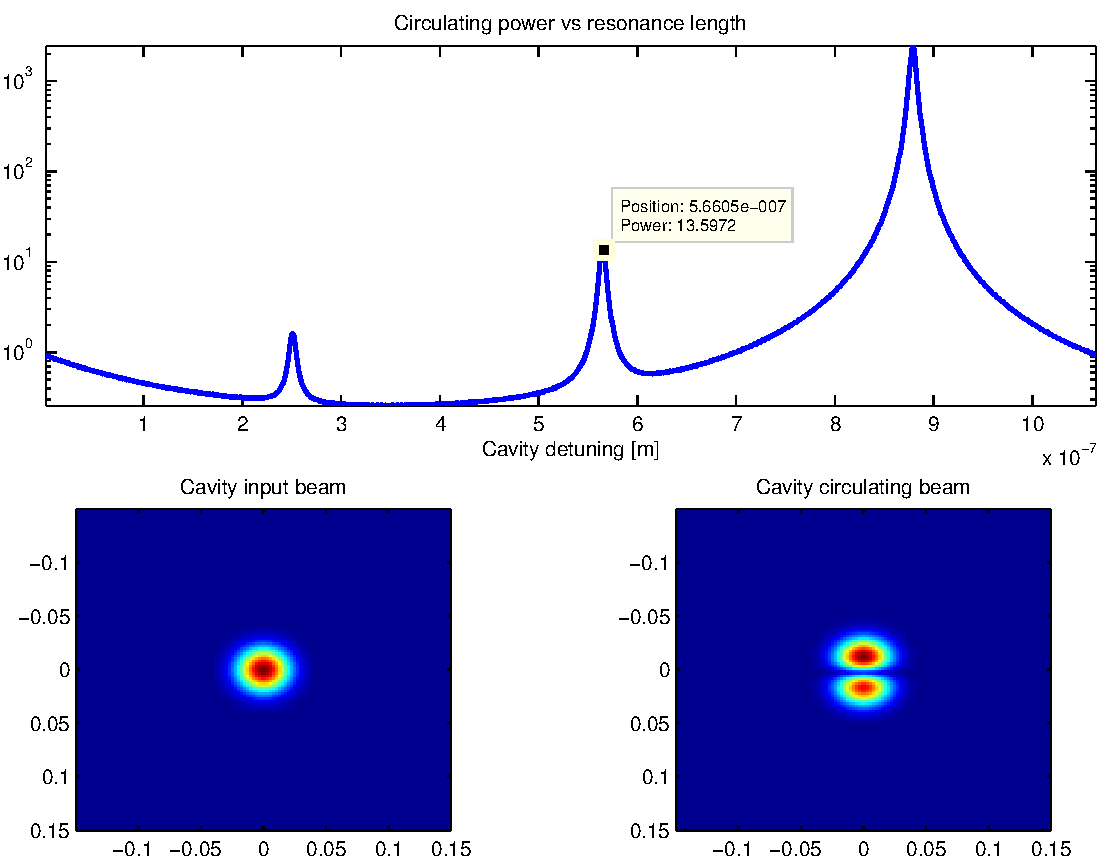
\includegraphics[width = 0.99\textwidth]{Fig5_scan.pdf}
\end{center}
\caption{\label{fig4:scan} Output window of the function \emph{Display\_scan(C1)} with the cavity scan over one FSR on top.}
\end{figure}

\section{Mirror maps and higher order modes}

In this example, we will demonstrate how to use higher order optical modes in conjunction with mirror maps. The mirror maps are stored in text files under the form of a matrix which represents the mirror height fluctuations in meter. In the maps given, the mirror curvature is not included (but it could be done). The RMS of the mirror maps is around 2~nm, typical of very good large mirrors.

The laser beam is now defined outside the cavity, so the cavity reflected field can also be calculated. The script for this example is called \textcolor{blue}{Example\_HOM\_with\_maps.m} and is shown in the listing \ref{lis4:cav_HOM} without any comments.\\

\begin{lstlisting}[float=htp,caption=Example of OSCAR script to calculate the reflected field from a cavity with maps \label{lis4:cav_HOM},frame=lines]
G1 = Grid(512,0.4);
E_input = E_Field(G1,0.043,-1034,'LG',3,3);

IM = Interface(G1,1500,0.35,0.02,0);
EM = Interface(G1,1700,0.35,0.02,0);

IM = Add_map(IM,'Map1.txt',1.5E-3);
EM = Add_map(EM,'Map2.txt',1.5E-3);

C1 = Cavity1(IM,EM,3000,E_input);
C1.Laser_start_on_input = false ;

C1 = Cavity_resonance_phase(C1);

C1 = Calculate_fields(C1);
Display_results(C1);
\end{lstlisting}

The line \verb|IM = Add_map(IM,'Map1.txt',1.5E-3)| is used to add the custom 2D map to the surface \verb|IM|. The map does not have to have the same size of the grid since internally an interpolation is done. The third argument \verb|1.5E-3| is the step size of the map in meter. The map can be normalise to a certain RMS by including a fourth argument such as: \verb|IM = Add_map(IM,'Map1.txt',1.5E-3,1E-9)|. In that case the map is automatically normalise to have a RMS of 1~nm.
Regarding the sign convention, positive values in the mirror maps reduce the length of the cavity.\\

After the definition of the cavity and the calculation of the resonance length, the command \verb|C1 = Calculate_fields(C1)| is used to calculate the circulating, reflected and transmitted fields from the cavity. The fields are then stored in the instance \verb|C1| where they could be access later. To display the result graphically the command \verb|Display_results(C1)| is then used. An example of the output screen is shown in figure \ref{fig5:LG33}

\begin{figure}
\begin{center}
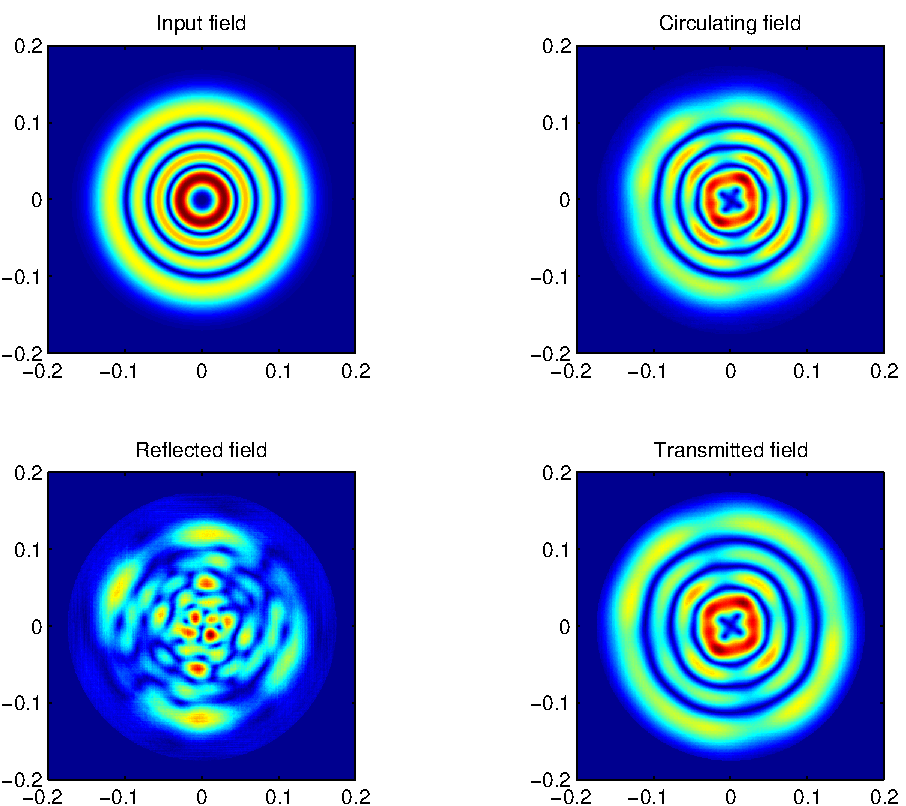
\includegraphics[width = 0.99\textwidth]{Fig5_Ref_LG.pdf}
\end{center}
\caption{\label{fig5:LG33} Output window of the function \emph{Display\_results(C1)} when a LG33 mode is expected to circulate in a cavity with realistic mirrors.}
\end{figure}

\clearpage
\section{Plotting Pound Drever Hall error signal} \label{ch4:ex_PDH}

In this example, we will learn how to create sidebands and derive a Pound Drever Hall locking signal in reflection. After the input laser \verb|E1| is defined, a virtual phase modulator creates a pair of sidebands with the command: \verb|E_input = Add_sidebands(E_input,6.7234E6,0.3)| (sideband frequency: 6.7234\,MHz and modulation depth: 0.3\,. Then the fields inside the cavity are computed for a given resonance phase.\\

To draw the PDH error signals, the reflected field from the cavity is demodulated to get the in phase and in quadrature signals. The simulation is relatively long since for the cavity scan 200 points are taken. That takes around 12 minutes on my laptop. A plot of the circulating power and the reflected PDH error signal is shown in figure \ref{fig5:PDH}.

\begin{figure}
\begin{center}
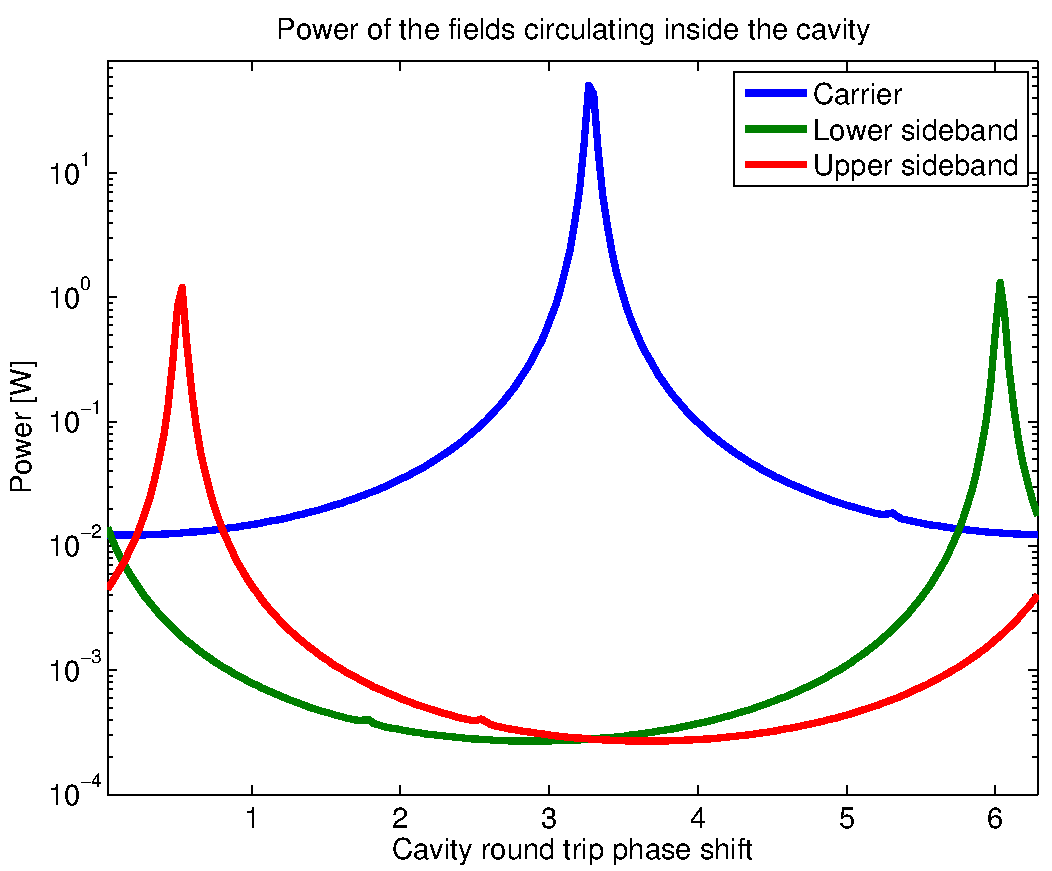
\includegraphics[width = 0.485\textwidth]{Fig5_PDH_circ.pdf}\hfill
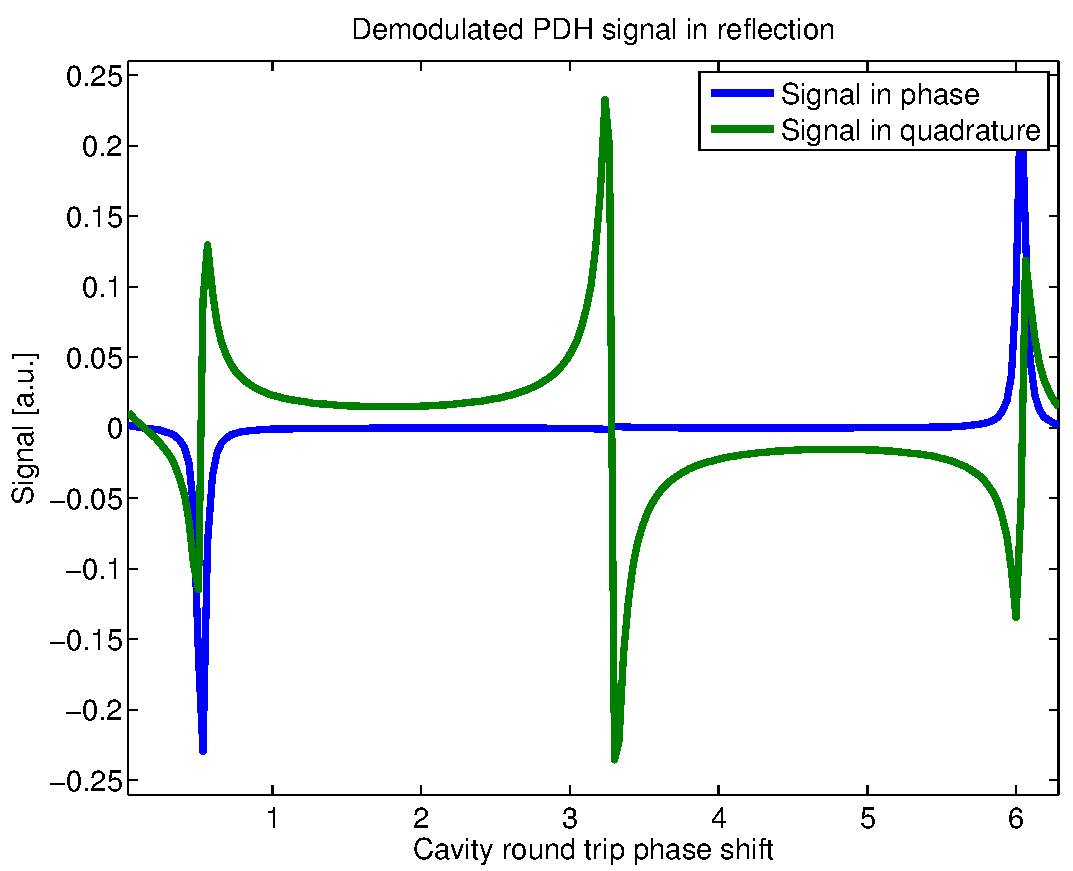
\includegraphics[width = 0.495\textwidth]{Fig5_PDH_ES.pdf}
\end{center}
\caption{\label{fig5:PDH} Circulating power inside the cavity (left) and error signals in reflection (right).}
\end{figure}

\section{4 mirrors linear cavity} \label{ch4:ex_OMC}

This example, introduces with OSCAR 3.05, shows how to simulate a 4 mirrors cavity. The parameters to define the cavity are taken from the GEO600 output mode cleaner. The script file is called \textcolor{blue}{Example\_4mirrors.m} and is rather self-explanatory for the regular user.

\section{Calculating the eigen modes of a Fabry-Perot cavity} \label{ch4:ex_OMC}

Since OSCAR V3.10, it is possible to calculate the eigens mode of a Fabry Perot or any linear cavity such as a mode cleaner. This particularly useful to check the degeneracy of a cavity or the clipping loss of higher order modes. The example file is called \textcolor{blue}{Example\_cavity\_eigenmodes.m}.

A typical display of the calculation of the cavity eigen modes is shown in figure \ref{fig5:cav_EM}.  Also, in this example file, at the end, it is shown how to display the Airy peak of the different higher order modes of the cavity.

\begin{figure}
\begin{center}
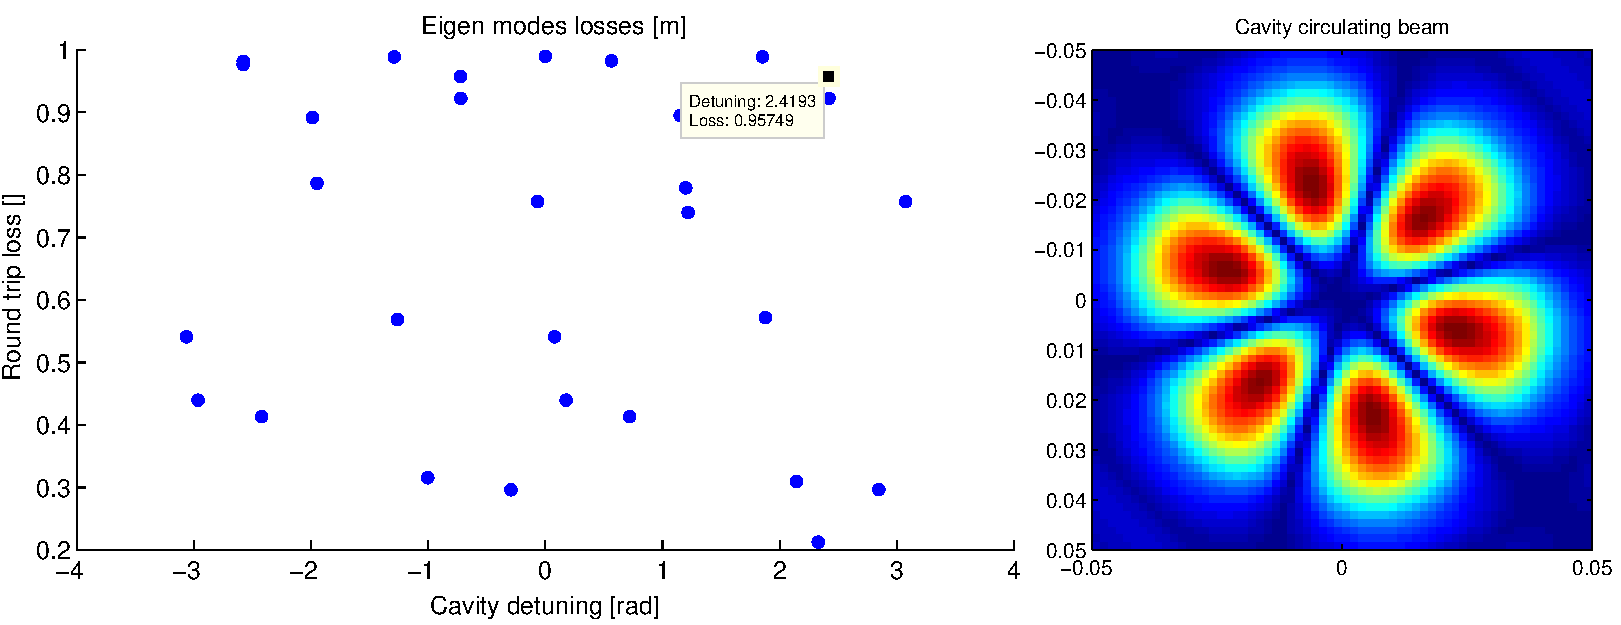
\includegraphics[width = 1.0\textwidth]{Fig5_cavity_EM.pdf}\hfill
\end{center}
\caption{\label{fig5:cav_EM} Result of the command \textcolor{blue}{Display\_cavity\_modes()}.}
\end{figure}

% FAQ
% Version 2.0 ?
% Change the accurary
